% Created by tikzDevice version 0.12.6 on 2024-11-19 16:55:39
% !TEX encoding = UTF-8 Unicode
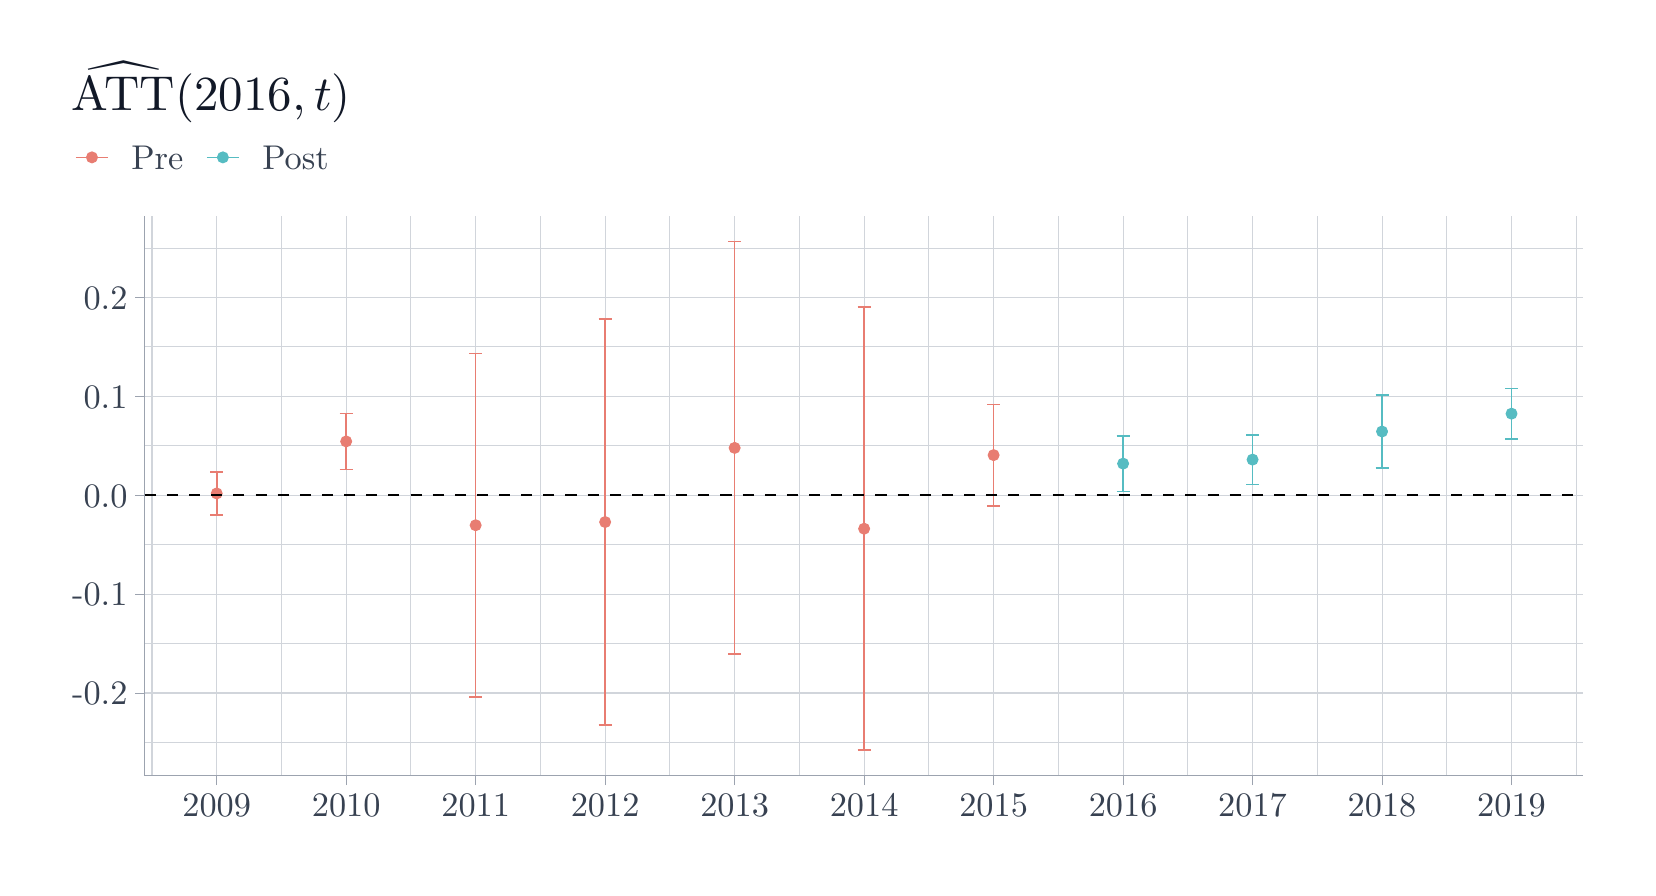
\begin{tikzpicture}[x=1pt,y=1pt]
\definecolor{fillColor}{RGB}{255,255,255}
\path[use as bounding box,fill=fillColor] (0,0) rectangle (578.16,303.53);
\begin{scope}
\path[clip] (  0.00,  0.00) rectangle (578.16,303.53);
\definecolor{drawColor}{RGB}{255,255,255}

\path[draw=drawColor,line width= 0.7pt,line join=round,line cap=round,fill=fillColor] (  0.00,  0.00) rectangle (578.16,303.53);
\end{scope}
\begin{scope}
\path[clip] ( 42.34, 33.29) rectangle (562.16,235.43);
\definecolor{drawColor}{RGB}{255,255,255}
\definecolor{fillColor}{RGB}{255,255,255}

\path[draw=drawColor,line width= 0.7pt,line join=round,line cap=round,fill=fillColor] ( 42.34, 33.29) rectangle (562.16,235.43);
\definecolor{drawColor}{RGB}{209,213,219}

\path[draw=drawColor,line width= 0.4pt,line join=round] ( 42.34, 45.25) --
	(562.16, 45.25);

\path[draw=drawColor,line width= 0.4pt,line join=round] ( 42.34, 80.98) --
	(562.16, 80.98);

\path[draw=drawColor,line width= 0.4pt,line join=round] ( 42.34,116.71) --
	(562.16,116.71);

\path[draw=drawColor,line width= 0.4pt,line join=round] ( 42.34,152.43) --
	(562.16,152.43);

\path[draw=drawColor,line width= 0.4pt,line join=round] ( 42.34,188.16) --
	(562.16,188.16);

\path[draw=drawColor,line width= 0.4pt,line join=round] ( 42.34,223.89) --
	(562.16,223.89);

\path[draw=drawColor,line width= 0.4pt,line join=round] ( 44.91, 33.29) --
	( 44.91,235.43);

\path[draw=drawColor,line width= 0.4pt,line join=round] ( 91.70, 33.29) --
	( 91.70,235.43);

\path[draw=drawColor,line width= 0.4pt,line join=round] (138.49, 33.29) --
	(138.49,235.43);

\path[draw=drawColor,line width= 0.4pt,line join=round] (185.28, 33.29) --
	(185.28,235.43);

\path[draw=drawColor,line width= 0.4pt,line join=round] (232.07, 33.29) --
	(232.07,235.43);

\path[draw=drawColor,line width= 0.4pt,line join=round] (278.85, 33.29) --
	(278.85,235.43);

\path[draw=drawColor,line width= 0.4pt,line join=round] (325.64, 33.29) --
	(325.64,235.43);

\path[draw=drawColor,line width= 0.4pt,line join=round] (372.43, 33.29) --
	(372.43,235.43);

\path[draw=drawColor,line width= 0.4pt,line join=round] (419.22, 33.29) --
	(419.22,235.43);

\path[draw=drawColor,line width= 0.4pt,line join=round] (466.01, 33.29) --
	(466.01,235.43);

\path[draw=drawColor,line width= 0.4pt,line join=round] (512.80, 33.29) --
	(512.80,235.43);

\path[draw=drawColor,line width= 0.4pt,line join=round] (559.59, 33.29) --
	(559.59,235.43);

\path[draw=drawColor,line width= 0.4pt,line join=round] ( 42.34, 63.12) --
	(562.16, 63.12);

\path[draw=drawColor,line width= 0.4pt,line join=round] ( 42.34, 98.84) --
	(562.16, 98.84);

\path[draw=drawColor,line width= 0.4pt,line join=round] ( 42.34,134.57) --
	(562.16,134.57);

\path[draw=drawColor,line width= 0.4pt,line join=round] ( 42.34,170.30) --
	(562.16,170.30);

\path[draw=drawColor,line width= 0.4pt,line join=round] ( 42.34,206.03) --
	(562.16,206.03);

\path[draw=drawColor,line width= 0.4pt,line join=round] ( 68.31, 33.29) --
	( 68.31,235.43);

\path[draw=drawColor,line width= 0.4pt,line join=round] (115.09, 33.29) --
	(115.09,235.43);

\path[draw=drawColor,line width= 0.4pt,line join=round] (161.88, 33.29) --
	(161.88,235.43);

\path[draw=drawColor,line width= 0.4pt,line join=round] (208.67, 33.29) --
	(208.67,235.43);

\path[draw=drawColor,line width= 0.4pt,line join=round] (255.46, 33.29) --
	(255.46,235.43);

\path[draw=drawColor,line width= 0.4pt,line join=round] (302.25, 33.29) --
	(302.25,235.43);

\path[draw=drawColor,line width= 0.4pt,line join=round] (349.04, 33.29) --
	(349.04,235.43);

\path[draw=drawColor,line width= 0.4pt,line join=round] (395.83, 33.29) --
	(395.83,235.43);

\path[draw=drawColor,line width= 0.4pt,line join=round] (442.61, 33.29) --
	(442.61,235.43);

\path[draw=drawColor,line width= 0.4pt,line join=round] (489.40, 33.29) --
	(489.40,235.43);

\path[draw=drawColor,line width= 0.4pt,line join=round] (536.19, 33.29) --
	(536.19,235.43);
\definecolor{drawColor}{RGB}{232,125,114}
\definecolor{fillColor}{RGB}{232,125,114}

\path[draw=drawColor,line width= 0.4pt,line join=round,line cap=round,fill=fillColor] ( 68.31,135.22) circle (  1.96);

\path[draw=drawColor,line width= 0.4pt,line join=round,line cap=round,fill=fillColor] (115.09,154.02) circle (  1.96);

\path[draw=drawColor,line width= 0.4pt,line join=round,line cap=round,fill=fillColor] (161.88,123.73) circle (  1.96);

\path[draw=drawColor,line width= 0.4pt,line join=round,line cap=round,fill=fillColor] (208.67,124.89) circle (  1.96);

\path[draw=drawColor,line width= 0.4pt,line join=round,line cap=round,fill=fillColor] (255.46,151.68) circle (  1.96);

\path[draw=drawColor,line width= 0.4pt,line join=round,line cap=round,fill=fillColor] (302.25,122.48) circle (  1.96);

\path[draw=drawColor,line width= 0.4pt,line join=round,line cap=round,fill=fillColor] (349.04,149.07) circle (  1.96);
\definecolor{drawColor}{RGB}{86,188,194}
\definecolor{fillColor}{RGB}{86,188,194}

\path[draw=drawColor,line width= 0.4pt,line join=round,line cap=round,fill=fillColor] (395.83,146.00) circle (  1.96);

\path[draw=drawColor,line width= 0.4pt,line join=round,line cap=round,fill=fillColor] (442.61,147.45) circle (  1.96);

\path[draw=drawColor,line width= 0.4pt,line join=round,line cap=round,fill=fillColor] (489.40,157.60) circle (  1.96);

\path[draw=drawColor,line width= 0.4pt,line join=round,line cap=round,fill=fillColor] (536.19,164.05) circle (  1.96);
\definecolor{drawColor}{RGB}{232,125,114}

\path[draw=drawColor,line width= 0.6pt,line join=round] ( 65.97,143.05) --
	( 70.64,143.05);

\path[draw=drawColor,line width= 0.6pt,line join=round] ( 68.31,143.05) --
	( 68.31,127.39);

\path[draw=drawColor,line width= 0.6pt,line join=round] ( 65.97,127.39) --
	( 70.64,127.39);

\path[draw=drawColor,line width= 0.6pt,line join=round] (112.75,164.13) --
	(117.43,164.13);

\path[draw=drawColor,line width= 0.6pt,line join=round] (115.09,164.13) --
	(115.09,143.91);

\path[draw=drawColor,line width= 0.6pt,line join=round] (112.75,143.91) --
	(117.43,143.91);

\path[draw=drawColor,line width= 0.6pt,line join=round] (159.54,185.79) --
	(164.22,185.79);

\path[draw=drawColor,line width= 0.6pt,line join=round] (161.88,185.79) --
	(161.88, 61.66);

\path[draw=drawColor,line width= 0.6pt,line join=round] (159.54, 61.66) --
	(164.22, 61.66);

\path[draw=drawColor,line width= 0.6pt,line join=round] (206.33,198.16) --
	(211.01,198.16);

\path[draw=drawColor,line width= 0.6pt,line join=round] (208.67,198.16) --
	(208.67, 51.62);

\path[draw=drawColor,line width= 0.6pt,line join=round] (206.33, 51.62) --
	(211.01, 51.62);

\path[draw=drawColor,line width= 0.6pt,line join=round] (253.12,226.24) --
	(257.80,226.24);

\path[draw=drawColor,line width= 0.6pt,line join=round] (255.46,226.24) --
	(255.46, 77.13);

\path[draw=drawColor,line width= 0.6pt,line join=round] (253.12, 77.13) --
	(257.80, 77.13);

\path[draw=drawColor,line width= 0.6pt,line join=round] (299.91,202.48) --
	(304.59,202.48);

\path[draw=drawColor,line width= 0.6pt,line join=round] (302.25,202.48) --
	(302.25, 42.47);

\path[draw=drawColor,line width= 0.6pt,line join=round] (299.91, 42.47) --
	(304.59, 42.47);

\path[draw=drawColor,line width= 0.6pt,line join=round] (346.70,167.35) --
	(351.38,167.35);

\path[draw=drawColor,line width= 0.6pt,line join=round] (349.04,167.35) --
	(349.04,130.80);

\path[draw=drawColor,line width= 0.6pt,line join=round] (346.70,130.80) --
	(351.38,130.80);
\definecolor{drawColor}{RGB}{86,188,194}

\path[draw=drawColor,line width= 0.6pt,line join=round] (393.49,156.02) --
	(398.17,156.02);

\path[draw=drawColor,line width= 0.6pt,line join=round] (395.83,156.02) --
	(395.83,135.98);

\path[draw=drawColor,line width= 0.6pt,line join=round] (393.49,135.98) --
	(398.17,135.98);

\path[draw=drawColor,line width= 0.6pt,line join=round] (440.28,156.44) --
	(444.95,156.44);

\path[draw=drawColor,line width= 0.6pt,line join=round] (442.61,156.44) --
	(442.61,138.46);

\path[draw=drawColor,line width= 0.6pt,line join=round] (440.28,138.46) --
	(444.95,138.46);

\path[draw=drawColor,line width= 0.6pt,line join=round] (487.06,170.70) --
	(491.74,170.70);

\path[draw=drawColor,line width= 0.6pt,line join=round] (489.40,170.70) --
	(489.40,144.49);

\path[draw=drawColor,line width= 0.6pt,line join=round] (487.06,144.49) --
	(491.74,144.49);

\path[draw=drawColor,line width= 0.6pt,line join=round] (533.85,173.14) --
	(538.53,173.14);

\path[draw=drawColor,line width= 0.6pt,line join=round] (536.19,173.14) --
	(536.19,154.96);

\path[draw=drawColor,line width= 0.6pt,line join=round] (533.85,154.96) --
	(538.53,154.96);
\definecolor{drawColor}{RGB}{0,0,0}

\path[draw=drawColor,line width= 0.6pt,dash pattern=on 4pt off 4pt ,line join=round] ( 42.34,134.57) -- (562.16,134.57);
\end{scope}
\begin{scope}
\path[clip] (  0.00,  0.00) rectangle (578.16,303.53);
\definecolor{drawColor}{RGB}{156,163,175}

\path[draw=drawColor,line width= 0.3pt,line join=round] ( 42.34, 33.29) --
	( 42.34,235.43);
\end{scope}
\begin{scope}
\path[clip] (  0.00,  0.00) rectangle (578.16,303.53);
\definecolor{drawColor}{RGB}{55,65,81}

\node[text=drawColor,anchor=base east,inner sep=0pt, outer sep=0pt, scale=  1.24] at ( 36.04, 58.83) {-0.2};

\node[text=drawColor,anchor=base east,inner sep=0pt, outer sep=0pt, scale=  1.24] at ( 36.04, 94.56) {-0.1};

\node[text=drawColor,anchor=base east,inner sep=0pt, outer sep=0pt, scale=  1.24] at ( 36.04,130.29) {0.0};

\node[text=drawColor,anchor=base east,inner sep=0pt, outer sep=0pt, scale=  1.24] at ( 36.04,166.01) {0.1};

\node[text=drawColor,anchor=base east,inner sep=0pt, outer sep=0pt, scale=  1.24] at ( 36.04,201.74) {0.2};
\end{scope}
\begin{scope}
\path[clip] (  0.00,  0.00) rectangle (578.16,303.53);
\definecolor{drawColor}{RGB}{156,163,175}

\path[draw=drawColor,line width= 0.3pt,line join=round] ( 38.84, 63.12) --
	( 42.34, 63.12);

\path[draw=drawColor,line width= 0.3pt,line join=round] ( 38.84, 98.84) --
	( 42.34, 98.84);

\path[draw=drawColor,line width= 0.3pt,line join=round] ( 38.84,134.57) --
	( 42.34,134.57);

\path[draw=drawColor,line width= 0.3pt,line join=round] ( 38.84,170.30) --
	( 42.34,170.30);

\path[draw=drawColor,line width= 0.3pt,line join=round] ( 38.84,206.03) --
	( 42.34,206.03);
\end{scope}
\begin{scope}
\path[clip] (  0.00,  0.00) rectangle (578.16,303.53);
\definecolor{drawColor}{RGB}{156,163,175}

\path[draw=drawColor,line width= 0.3pt,line join=round] ( 42.34, 33.29) --
	(562.16, 33.29);
\end{scope}
\begin{scope}
\path[clip] (  0.00,  0.00) rectangle (578.16,303.53);
\definecolor{drawColor}{RGB}{156,163,175}

\path[draw=drawColor,line width= 0.3pt,line join=round] ( 68.31, 29.79) --
	( 68.31, 33.29);

\path[draw=drawColor,line width= 0.3pt,line join=round] (115.09, 29.79) --
	(115.09, 33.29);

\path[draw=drawColor,line width= 0.3pt,line join=round] (161.88, 29.79) --
	(161.88, 33.29);

\path[draw=drawColor,line width= 0.3pt,line join=round] (208.67, 29.79) --
	(208.67, 33.29);

\path[draw=drawColor,line width= 0.3pt,line join=round] (255.46, 29.79) --
	(255.46, 33.29);

\path[draw=drawColor,line width= 0.3pt,line join=round] (302.25, 29.79) --
	(302.25, 33.29);

\path[draw=drawColor,line width= 0.3pt,line join=round] (349.04, 29.79) --
	(349.04, 33.29);

\path[draw=drawColor,line width= 0.3pt,line join=round] (395.83, 29.79) --
	(395.83, 33.29);

\path[draw=drawColor,line width= 0.3pt,line join=round] (442.61, 29.79) --
	(442.61, 33.29);

\path[draw=drawColor,line width= 0.3pt,line join=round] (489.40, 29.79) --
	(489.40, 33.29);

\path[draw=drawColor,line width= 0.3pt,line join=round] (536.19, 29.79) --
	(536.19, 33.29);
\end{scope}
\begin{scope}
\path[clip] (  0.00,  0.00) rectangle (578.16,303.53);
\definecolor{drawColor}{RGB}{55,65,81}

\node[text=drawColor,anchor=base,inner sep=0pt, outer sep=0pt, scale=  1.24] at ( 68.31, 18.42) {2009};

\node[text=drawColor,anchor=base,inner sep=0pt, outer sep=0pt, scale=  1.24] at (115.09, 18.42) {2010};

\node[text=drawColor,anchor=base,inner sep=0pt, outer sep=0pt, scale=  1.24] at (161.88, 18.42) {2011};

\node[text=drawColor,anchor=base,inner sep=0pt, outer sep=0pt, scale=  1.24] at (208.67, 18.42) {2012};

\node[text=drawColor,anchor=base,inner sep=0pt, outer sep=0pt, scale=  1.24] at (255.46, 18.42) {2013};

\node[text=drawColor,anchor=base,inner sep=0pt, outer sep=0pt, scale=  1.24] at (302.25, 18.42) {2014};

\node[text=drawColor,anchor=base,inner sep=0pt, outer sep=0pt, scale=  1.24] at (349.04, 18.42) {2015};

\node[text=drawColor,anchor=base,inner sep=0pt, outer sep=0pt, scale=  1.24] at (395.83, 18.42) {2016};

\node[text=drawColor,anchor=base,inner sep=0pt, outer sep=0pt, scale=  1.24] at (442.61, 18.42) {2017};

\node[text=drawColor,anchor=base,inner sep=0pt, outer sep=0pt, scale=  1.24] at (489.40, 18.42) {2018};

\node[text=drawColor,anchor=base,inner sep=0pt, outer sep=0pt, scale=  1.24] at (536.19, 18.42) {2019};
\end{scope}
\begin{scope}
\path[clip] (  0.00,  0.00) rectangle (578.16,303.53);
\definecolor{drawColor}{RGB}{255,255,255}
\definecolor{fillColor}{RGB}{255,255,255}

\path[draw=drawColor,line width= 0.7pt,line join=round,line cap=round,fill=fillColor] ( 16.00,249.43) rectangle (108.85,263.89);
\end{scope}
\begin{scope}
\path[clip] (  0.00,  0.00) rectangle (578.16,303.53);
\definecolor{drawColor}{RGB}{255,255,255}
\definecolor{fillColor}{RGB}{255,255,255}

\path[draw=drawColor,line width= 0.7pt,line join=round,line cap=round,fill=fillColor] ( 16.00,249.43) rectangle ( 30.45,263.89);
\end{scope}
\begin{scope}
\path[clip] (  0.00,  0.00) rectangle (578.16,303.53);
\definecolor{drawColor}{RGB}{232,125,114}
\definecolor{fillColor}{RGB}{232,125,114}

\path[draw=drawColor,line width= 0.4pt,line join=round,line cap=round,fill=fillColor] ( 23.23,256.66) circle (  1.96);
\end{scope}
\begin{scope}
\path[clip] (  0.00,  0.00) rectangle (578.16,303.53);
\definecolor{drawColor}{RGB}{232,125,114}

\path[draw=drawColor,line width= 0.6pt,line join=round] ( 17.45,256.66) -- ( 29.01,256.66);
\end{scope}
\begin{scope}
\path[clip] (  0.00,  0.00) rectangle (578.16,303.53);
\definecolor{drawColor}{RGB}{255,255,255}
\definecolor{fillColor}{RGB}{255,255,255}

\path[draw=drawColor,line width= 0.7pt,line join=round,line cap=round,fill=fillColor] ( 63.32,249.43) rectangle ( 77.77,263.89);
\end{scope}
\begin{scope}
\path[clip] (  0.00,  0.00) rectangle (578.16,303.53);
\definecolor{drawColor}{RGB}{86,188,194}
\definecolor{fillColor}{RGB}{86,188,194}

\path[draw=drawColor,line width= 0.4pt,line join=round,line cap=round,fill=fillColor] ( 70.54,256.66) circle (  1.96);
\end{scope}
\begin{scope}
\path[clip] (  0.00,  0.00) rectangle (578.16,303.53);
\definecolor{drawColor}{RGB}{86,188,194}

\path[draw=drawColor,line width= 0.6pt,line join=round] ( 64.76,256.66) -- ( 76.33,256.66);
\end{scope}
\begin{scope}
\path[clip] (  0.00,  0.00) rectangle (578.16,303.53);
\definecolor{drawColor}{RGB}{55,65,81}

\node[text=drawColor,anchor=base west,inner sep=0pt, outer sep=0pt, scale=  1.24] at ( 37.45,252.37) {Pre};
\end{scope}
\begin{scope}
\path[clip] (  0.00,  0.00) rectangle (578.16,303.53);
\definecolor{drawColor}{RGB}{55,65,81}

\node[text=drawColor,anchor=base west,inner sep=0pt, outer sep=0pt, scale=  1.24] at ( 84.77,252.37) {Post};
\end{scope}
\begin{scope}
\path[clip] (  0.00,  0.00) rectangle (578.16,303.53);
\definecolor{drawColor}{RGB}{17,24,39}

\node[text=drawColor,anchor=base west,inner sep=0pt, outer sep=0pt, scale=  1.77] at ( 16.00,273.61) {$\widehat{\textrm{ATT}}(2016, t)$};
\end{scope}
\end{tikzpicture}
